\documentclass{beamer}
\mode<presentation>
\usepackage{amsmath}
\usepackage{amssymb}
%\usepackage{advdate}
\usepackage{adjustbox}
\usepackage{subcaption}
\usepackage{enumitem}
\usepackage{multicol}
\usepackage{mathtools}
\usepackage{listings}
\usepackage{url}
\usepackage{tikz}
\usetikzlibrary{matrix}
\def\UrlBreaks{\do\/\do-}
\usetheme{metropolis}
%\usecolortheme{lily}
\setbeamertemplate{footline}
{
  \leavevmode%
  \hbox{%
  \begin{beamercolorbox}[wd=\paperwidth,ht=2.25ex,dp=1ex,right]{author in head/foot}%
    \insertframenumber{} / \inserttotalframenumber\hspace*{2ex} 
  \end{beamercolorbox}}%
  \vskip0pt%
}
\setbeamertemplate{navigation symbols}{}

\providecommand{\nCr}[2]{\,^{#1}C_{#2}} % nCr
\providecommand{\nPr}[2]{\,^{#1}P_{#2}} % nPr
\providecommand{\mbf}{\mathbf}
\providecommand{\pr}[1]{\ensuremath{\Pr\left(#1\right)}}
\providecommand{\qfunc}[1]{\ensuremath{Q\left(#1\right)}}
\providecommand{\sbrak}[1]{\ensuremath{{}\left[#1\right]}}
\providecommand{\lsbrak}[1]{\ensuremath{{}\left[#1\right.}}
\providecommand{\rsbrak}[1]{\ensuremath{{}\left.#1\right]}}
\providecommand{\brak}[1]{\ensuremath{\left(#1\right)}}
\providecommand{\lbrak}[1]{\ensuremath{\left(#1\right.}}
\providecommand{\rbrak}[1]{\ensuremath{\left.#1\right)}}
\providecommand{\cbrak}[1]{\ensuremath{\left\{#1\right\}}}
\providecommand{\lcbrak}[1]{\ensuremath{\left\{#1\right.}}
\providecommand{\rcbrak}[1]{\ensuremath{\left.#1\right\}}}
\theoremstyle{remark}
\newtheorem{rem}{Remark}
\newcommand{\sgn}{\mathop{\mathrm{sgn}}}
\providecommand{\abs}[1]{\left\vert#1\right\vert}
\providecommand{\res}[1]{\Res\displaylimits_{#1}} 
\providecommand{\norm}[1]{\lVert#1\rVert}
\providecommand{\mtx}[1]{\mathbf{#1}}
\providecommand{\mean}[1]{E\left[ #1 \right]}
\providecommand{\fourier}{\overset{\mathcal{F}}{ \rightleftharpoons}}
%\providecommand{\hilbert}{\overset{\mathcal{H}}{ \rightleftharpoons}}
\providecommand{\system}{\overset{\mathcal{H}}{ \longleftrightarrow}}
	%\newcommand{\solution}[2]{\textbf{Solution:}{#1}}
%\newcommand{\solution}{\noindent \textbf{Solution: }}
\providecommand{\dec}[2]{\ensuremath{\overset{#1}{\underset{#2}{\gtrless}}}}
\newcommand{\myvec}[1]{\ensuremath{\begin{pmatrix}#1\end{pmatrix}}}
\let\vec\mathbf

\lstset{
%language=C,
frame=single, 
breaklines=true,
columns=fullflexible
}

\numberwithin{equation}{section}

\title{Computationally solving system of linear equations \brak{\text{10.3.3.1.3}}}
\author{Agamjot Singh,\\EE24BTECH11002,\\IIT Hyderabad.}

\date{\today} 
\begin{document}

\begin{frame}
\titlepage
\end{frame}

\section*{Outline}
\begin{frame}
\frametitle{Table of Contents}
\tableofcontents
\end{frame}

\section{Problem}

\begin{frame}
\frametitle{Problem Statement}
Solve the following pair of linear equations,
\begin{align}
    3x - y = 3\\
    9x - 3y = 9
\end{align}
\end{frame}

\section{Solution}

%Slide1
\subsection{Computation Solution - LU Decomposition Method}
\begin{frame}
\frametitle{Computation Solution - LU Decomposition Method}
Let
\begin{align}
    \vec{x} = \myvec{x\\y}
\end{align}
Expressing the system in matrix form,
\begin{align}
    \myvec{3 & -1\\9 & -3}\vec{x} = \myvec{3\\9}\\
    \text{which is of the form } A\vec{x} = \vec{b}
\end{align}
\end{frame}

%Slide2
\begin{frame}
Any non-singular matrix $A$ can be expressed as a product of an upper triangular matrix $U$ and a lower triangular matrix $L$, such that
\begin{align}
    A &= LU\\
    \implies LU\vec{x} &= \vec{b}
\end{align}
$U$ is determined by row reducing $A$,
\begin{align}
    \myvec{3 & -1\\9 & -3} \xrightarrow{R_2 \to R_2 - 3R_1} \myvec{3 & -1\\0 & 0}
\end{align}
Let 
\begin{align}
    L = \myvec{1 & 0\\l_{21} & 1}
\end{align}
$l_{21}$ is the multiplier used to zero out $a_{21}$ in $A$.
\begin{align}
    L = \myvec{1 & 0\\3 & 1}
\end{align}
\end{frame}

%Slide3
\begin{frame}
This $LU$ decomposition could also be computationally found using Doolittle's algorithm. The update equation is given by,
\begin{align}
    U_{ij} &= \begin{cases}
        A_{ij} & \quad i = 0\\
        A_{ij} - \sum_{k = 0}^{i - 1} L_{ik} U_{kj} & \quad i > 0
    \end{cases}\\
    L_{ij} &= \begin{cases}
        \frac{A_{ij}}{U_{jj}} & \quad j = 0, U_{jj} \neq 0\\
        \frac{A_{ij} - \sum_{k = 0}^{j - 1} L_{ik} U_{kj}}{U_{jj}} & \quad j > 0
    \end{cases}\\
\end{align}
\end{frame}

%Slide4
\begin{frame}
We see that there is a zero on the diagonal of the upper triangular matrix $U$ which implies that $A$ is singular and hence the system has either zero or infinitely many solutions.
\newline
Let $\vec{y} = U\vec{x}$,
\begin{align}
    L\vec{y} = \vec{b} \label{y_eq}
\end{align}
After we find $\vec{y}$, we find $\vec{x}$ using the following equation,
\begin{align}
    U\vec{x} = \vec{y} \label{x_eq}
\end{align}
Applying forward substitution on equation $\brak{\ref{y_eq}}$, we get,
\begin{align}
    \myvec{1 & 0\\3 & 1}\myvec{y_1\\y_2} &= \myvec{3\\9}\\
    \implies \myvec{y_1\\y_2} &= \myvec{3\\0}
\end{align}
\end{frame}

%Slide5
\begin{frame}
Substituting $\vec{y}$ in equation $\brak{\ref{x_eq}}$, we get,
\begin{align}
    \myvec{3 & -1\\0 & 0} \myvec{x\\y} &= \myvec{3\\0}\\
    \implies 0\brak{x} + 0\brak{y} &= 0\\
    \text{and } 3x - y &= 3
\end{align}
This shows that the equation has infinitely many solutions.
\end{frame}

%Slide6
\subsection{Plot}
\begin{frame}
\frametitle{Plot}
\begin{figure}[h!]
   \centering
   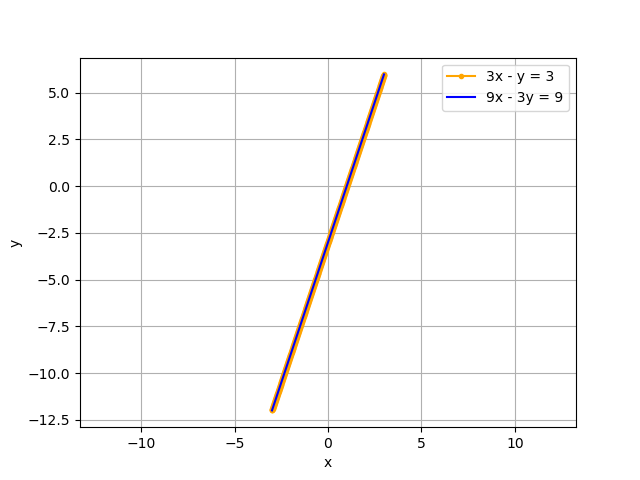
\includegraphics[width=0.7\linewidth]{figs/graph.png}
   \caption{Plotting the two lines, which come out as parallel}
\end{figure}
\end{frame}

\end{document}
